%%%%%%%%%%%%%%%%%%%%%%%%%%%%%%%%%%%%%%%%%
% Masters/Doctoral Thesis
% LaTeX Template
% Version 2.5 (27/8/17)
%
% This template was downloaded from:
% http://www.LaTeXTemplates.com
%
% Version 2.x major modifications by:
% Vel (vel@latextemplates.com)
%
% This template is based on a template by:
% Steve Gunn (http://users.ecs.soton.ac.uk/srg/softwaretools/document/templates/)
% Sunil Patel (http://www.sunilpatel.co.uk/thesis-template/)
%
% Template license:
% CC BY-NC-SA 3.0 (http://creativecommons.org/licenses/by-nc-sa/3.0/)
%
%%%%%%%%%%%%%%%%%%%%%%%%%%%%%%%%%%%%%%%%%

%----------------------------------------------------------------------------------------
%	PACKAGES AND OTHER DOCUMENT CONFIGURATIONS
%----------------------------------------------------------------------------------------
\documentclass[
11pt, % The default document font size, options: 10pt, 11pt, 12pt
oneside, % Two side (alternating margins) for binding by default, uncomment to switch to one side
english, % ngerman for German
singlespacing, % Single line spacing, alternatives: onehalfspacing or doublespacing
headsepline, % Uncomment to get a line under the header
chapterinoneline, % Uncomment to place the chapter title next to the number on one line
]{MastersDoctoralThesis} % The class file specifying the document structure

\usepackage[utf8]{inputenc} % Required for inputting international characters
\usepackage[T1]{fontenc} % Output font encoding for international characters
\usepackage{mathpazo} % Use the Palatino font by default
\usepackage{cite}

\usepackage[autostyle=true]{csquotes} % Required to generate language-dependent quotes in the bibliography

\usepackage{amstext, amsfonts, amsmath, amsbsy, amssymb}
\usepackage{tikz}
\usetikzlibrary{positioning, arrows.meta, fit}
\usepackage{booktabs}
\usepackage{caption}
\usepackage{subcaption}
\usepackage{easyReview}

%----------------------------------------------------------------------------------------
%	MARGIN SETTINGS
%----------------------------------------------------------------------------------------

\geometry{
	paper=a4paper, % Change to letterpaper for US letter
	inner=2.5cm, % Inner margin
	outer=3.8cm, % Outer margin
	bindingoffset=.5cm, % Binding offset
	top=1.5cm, % Top margin
	bottom=1.5cm, % Bottom margin
}

%----------------------------------------------------------------------------------------
%	THESIS INFORMATION
%----------------------------------------------------------------------------------------

\thesistitle{ACOL : Random Markov Field} % Your thesis title, this is used in the title and abstract, print it elsewhere with \ttitle
\supervisor{Prof. Daniel \textsc{Wegmann} \\ \& Dr. Pierre-Marie \textsc{Allard}}
\examiner{}
\degree{Master of Science in Bioinformatics and Computational Biology}
\author{Marco \textsc{Visani}}
\addresses{}

\subject{Biological Sciences}
\keywords{}
\university{\href{https://www.unifr.ch/}{University of Fribourg}}
\department{\href{https://www.unifr.ch/bio/en/}{Department of Biology}}
\group{\href{https://www.unifr.ch/bio/en/groups/wegmann/}{Wegmann Group} \& \href{https://www.unifr.ch/bio/en/groups/allard/}{COMMONS Lab}}
\faculty{\href{https://www.unifr.ch/scimed/en/}{Faculty of Science and Medicine}}

\AtBeginDocument{
\hypersetup{pdftitle=\ttitle} % Set the PDF's title to your title
\hypersetup{pdfauthor=\authorname} % Set the PDF's author to your name
\hypersetup{pdfkeywords=\keywordnames} % Set the PDF's keywords to your keywords
}


%----------------------------------------------------------------------------------------
%	MATH STUFF
\DeclareMathOperator{\Poisson}{Poisson}
\DeclareMathOperator{\Multinom}{Multinom}
\DeclareMathOperator{\logit}{logit}
\DeclareMathOperator{\cov}{cov}
\DeclareMathOperator{\Ind}{I}
\DeclareMathOperator{\Unif}{Uniform}
\DeclareMathOperator{\Normal}{Normal}
\DeclareMathOperator{\GammaDist}{Gamma}
\DeclareMathOperator{\BetaDist}{Beta}
\DeclareMathOperator{\Exponential}{Exp}
\DeclareMathOperator{\Bernoulli}{Bernoulli}
\def\P{\mathbb{P}}

\def\x{\boldsymbol{x}}

\def\btau{\boldsymbol{\tau}}
\def\bmu{\boldsymbol{\mu}}
\def\bxi{\boldsymbol{\xi}}
\def\bLambda{\boldsymbol{\Lambda}}
\def\bP{\boldsymbol{P}}
\def\bPi{\boldsymbol{\Pi}}
\def\bd{\boldsymbol{d}}
\def\btheta{\boldsymbol{\theta}}

\def\Ccal{{\cal C}}
\def\C{{\cal C}}
\def\E{{\cal E}}
\def\I{{\cal I}}
\def\N{{\cal N}}
\def\M{{\cal M}}
\def\R{{\cal R}}
\def\T{{\cal T}}
\def\X{{\cal X}}
\def\Y{{\cal Y}}
\def\Z{{\cal Z}}
\def\D{{\cal D}}
\def\F{{\cal F}}
\def\J{{\cal J}}
\def\Jin{\J^{\mathrm{in}}}
\def\Jout{\J^{\mathrm{out}}}

%----------------------------------------------------------------------------------------

\linespread{1.25}
\begin{document}


\frontmatter % Use roman page numbering style (i, ii, iii, iv...) for the pre-content pages

\pagestyle{plain} % Default to the plain heading style until the thesis style is called for the body content

%----------------------------------------------------------------------------------------
%	TITLE PAGE
%----------------------------------------------------------------------------------------

\begin{titlepage}
	
\includegraphics[scale=0.3]{images/UnifrLogo} % University logo
	\begin{center}
		\vspace*{.06\textheight}
		{\scshape\LARGE \univname\par}\vspace{1.5cm} % University name

		\textsc{\Large Manuscript}\\[0.5cm] % Thesis type

		\HRule \\[0.4cm] % Horizontal line
		{\huge \bfseries \ttitle\par}\vspace{0.4cm} % Thesis title
		\HRule \\[1.5cm] % Horizontal line

		\begin{minipage}[t]{0.4\textwidth}
			\begin{flushleft} \large
				\emph{Authors:}\\
				\href{mailto:madleina.caduff@unifr.ch}{Madleina \textsc{Caduff}}\\
				\href{mailto:contact@vismarco.ch}{\authorname}
			\end{flushleft}
		\end{minipage}
		\begin{minipage}[t]{0.4\textwidth}
			\begin{flushright} \large
				\emph{Supervisors:} \\
				\href{mailto:daniel.wegmann@unifr.ch}{Prof. Daniel \textsc{Wegmann}} \\
				\href{mailto:pierre-marie.allard@unifr.ch}{Dr. Pierre-Marie \textsc{Allard}}
			\end{flushright}
		\end{minipage}\\[3cm]

		\vfill
		\vfill

		{\large \today}\\[4cm] % Date

		\vfill
	\end{center}
\end{titlepage}

%----------------------------------------------------------------------------------------
%	LIST OF CONTENTS/FIGURES/TABLES PAGES
%----------------------------------------------------------------------------------------

\tableofcontents % Prints the main table of contents

%----------------------------------------------------------------------------------------
%	ABBREVIATIONS
%----------------------------------------------------------------------------------------
%
\begin{abbreviations}{ll}\label{sec:abbreviations}

	\textbf{CTMC} & \textbf{C}ontinuous-\textbf{T}ime \textbf{M}arkov \textbf{C}hain\\
	\textbf{DAG} & \textbf{D}irected \textbf{A}cyclic \textbf{G}raph\\
	\textbf{LC-MSMS} & \textbf{L}iquid \textbf{C}hromatography -- tandem \textbf{M}ass \textbf{S}pectrometry\\
	\textbf{LR} & \textbf{L}ikelihood \textbf{R}atio\\
	\textbf{MCMC} & \textbf{M}arkov \textbf{C}hain \textbf{M}onte \textbf{C}arlo\\
	\textbf{MH} & \textbf{M}etropolis--\textbf{H}astings\\
	\textbf{MS} & \textbf{M}ass \textbf{S}pectrometry \\
	\textbf{NP(s)} & \textbf{N}atural \textbf{P}roduct(s) \\
	\textbf{RMF} & \textbf{R}andom \textbf{M}arkov \textbf{F}ield \\

\end{abbreviations}


%----------------------------------------------------------------------------------------
%	THESIS CONTENT - CHAPTERS
%----------------------------------------------------------------------------------------

\mainmatter % Begin numeric (1,2,3...) page numbering

\pagestyle{thesis} % Return the page headers back to the "thesis" style

\chapter{Random Markov Field}
\section{Model}

We seek to infer the presence or absence of NPs across species. We assume that the pattern of presence and absence is modulated by similarities along two dimensions: closely related species may share a similar set of NPs, and NPs related in their synthesis may share a similar distribution across species. Each dimension is described by a known tree, and presence and absence evolve along each tree as a Markov process. Information flows between the two trees only through the leaf level, where each pair of a species and an NP has one presence state (Figure~\ref{fig:dag}).

\paragraph{Trees} We consider two dimensions: the species $s$ and the NPs $m$. Each dimension $d \in \{s, m\}$ consists of a set $\E_d$ of discrete entries, the leaves: $S = |\E_s|$ species and $M = |\E_m|$ NPs. We model similarities between the entries of dimension $d$ using a Markov process along a known tree $\T_d$ consisting of $\N_d = \E_d \cup \R_d \cup \I_d$ nodes: the entries $\E_d$ are leaves, connected to the set of roots $\R_d$ through a set of internal nodes $\I_d$. A tree may have several roots, and every root has at least one child. For every node $n \in \N_d \setminus \R_d$, let $p(n) \in \N_d$ denote its parent node and $b(n) > 0$ the length of the branch connecting it to its parent. Throughout, $i \in \E_s$ denotes a species leaf and $j \in \E_m$ an NP leaf.

\paragraph{Node states and cliques} Every node of a tree carries one binary presence state for every leaf of the other tree. Along the species tree, $Z^s_{nj} \in \{0,1\}$ is the state of species node $n \in \N_s$ for NP leaf $j \in \E_m$; along the NP tree, $Z^m_{in} \in \{0,1\}$ is the state of NP node $n \in \N_m$ for species leaf $i \in \E_s$. We write $\Z^s = (Z^s_{nj})$, an $|\N_s| \times M$ array, and $\Z^m = (Z^m_{in})$, an $S \times |\N_m|$ array, and call them the \emph{node states} of each tree.

The node states factorize over a set of \href{https://en.wikipedia.org/wiki/Clique_(graph_theory)}{cliques} $\C = \C_s \cup \C_m$. A clique $c \in \C_s$ consists of the states of all nodes of $\T_s$ for one fixed NP leaf $j$, $c^s_j = \{Z^s_{nj} : n \in \N_s\}$; a clique $c \in \C_m$ consists of the states of all nodes of $\T_m$ for one fixed species leaf $i$, $c^m_i = \{Z^m_{in} : n \in \N_m\}$. We refer to the tree a clique varies along, $v(c) \in \{s, m\}$, as its \emph{variable} dimension. There are $M$ cliques along the species tree and $S$ cliques along the NP tree, and no two cliques share a variable.

\paragraph{Tree fields and the field} The node states extend down to the leaves of their own tree. The leaf block of each tree,
\begin{equation*}
	Z^s_{ij},\ i \in \E_s,\ j \in \E_m \qquad\text{and}\qquad Z^m_{ij},\ i \in \E_s,\ j \in \E_m,
\end{equation*}
is an $S \times M$ array that we call the \emph{tree field} of that tree. Each tree field is the view of one tree on the leaf level. The presence of NP $j$ in species $i$ is a third variable, $Y_{ij} \in \{0,1\}$, and we call the $S \times M$ array $\Y = (Y_{ij})$ the \emph{field}. The field is drawn from the two tree fields by a link with a single parameter, described below. The latent variables of the model are then $\X = \Y \cup \Z^s \cup \Z^m$.

Keeping three variables per leaf pair rather than one is what makes the joint density proper. If both trees instead shared a single leaf variable, as an undirected product of the clique functions of both trees would require, the normalizing constant of that product,
\begin{equation*}
	C(\btheta_s, \btheta_m) = \sum_{\Y} \P_s(\Y \mid \btheta_s)\, \P_m(\Y \mid \btheta_m),
\end{equation*}
where $\P_d(\Y \mid \btheta_d)$ is the marginal probability of the leaf states along tree $d$, would depend on the parameters and be a sum over $2^{SM}$ fields. Ignoring it, as any MCMC on the tree parameters must, targets $\P(\btheta)\,C(\btheta)$ instead of the posterior. Because $C$ grows as the two trees' leaf distributions concentrate on the same fields, it pulls the switching rates towards zero. On simulated data this placed the posterior of $\log \nu$ up to $1.4$ below the truth on a $4 \times 4$ field and made it diverge on larger ones. Under the factorization below every factor is a conditional density, and the joint density sums to one for every value of the parameters.

\begin{figure}
	\centering
	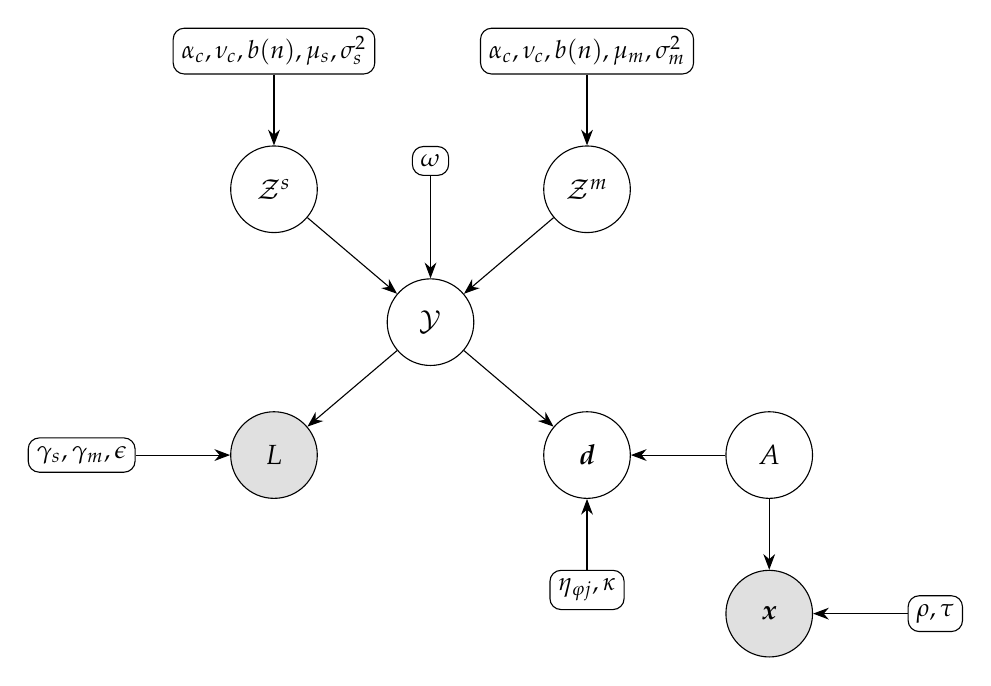
\begin{tikzpicture}[
		var/.style={circle, draw, minimum size=11mm, inner sep=0pt},
		obs/.style={var, fill=black!12},
		par/.style={rectangle, draw, rounded corners, inner sep=3pt, font=\small},
		->, >={Stealth[length=2mm]}, node distance=9mm and 12mm]
		\node[var] (Y) {$\Y$};
		\node[var, above left=of Y] (Zs) {$\Z^s$};
		\node[var, above right=of Y] (Zm) {$\Z^m$};
		\node[par, above=of Zs] (ts) {$\alpha_c, \nu_c, b(n), \mu_s, \sigma^2_s$};
		\node[par, above=of Zm] (tm) {$\alpha_c, \nu_c, b(n), \mu_m, \sigma^2_m$};
		\node[par, above=13mm of Y] (om) {$\omega$};
		\node[obs, below left=of Y] (L) {$L$};
		\node[var, below right=of Y] (d) {$\bd$};
		\node[var, right=of d] (A) {$A$};
		\node[obs, below=of A] (xs) {$\x$};
		\node[par, left=of L] (lp) {$\gamma_s, \gamma_m, \epsilon$};
		\node[par, below=of d] (dp) {$\eta_{\varphi j}, \kappa$};
		\node[par, right=of xs] (xp) {$\rho, \tau$};
		\draw (ts) -- (Zs);
		\draw (tm) -- (Zm);
		\draw (Zs) -- (Y);
		\draw (Zm) -- (Y);
		\draw (om) -- (Y);
		\draw (Y) -- (L);
		\draw (lp) -- (L);
		\draw (Y) -- (d);
		\draw (dp) -- (d);
		\draw (A) -- (d);
		\draw (A) -- (xs);
		\draw (xp) -- (xs);
	\end{tikzpicture}
	\caption{The model as a directed graph. Each tree generates its node states $\Z^s$, $\Z^m$, whose leaf blocks are the two tree fields. The field $\Y$ is a noisy AND of the tree fields. LOTUS records $L$ and the LC-MSMS data inform the field. For LC-MSMS, the detections $\bd$ are a function of the latent assignments $A$ of features to NPs, and the feature scores $\x$ inform the assignments. Shaded nodes are observed; boxes are parameters.}
	\label{fig:dag}
\end{figure}

\paragraph{Markov model along trees} We model each clique using a two-state CTMC along the tree of its variable dimension. Let
\begin{equation}
	\bLambda_c = \nu_c
	\begin{pmatrix}
		-\alpha_c  & \alpha_c    \\
		1-\alpha_c & -(1-\alpha_c) \\
	\end{pmatrix}
\end{equation}
be the rate matrix for changes between states 0 and 1 along the tree, where $\alpha_c \in (0,1)$ is the stationary frequency of presence and $\nu_c > 0$ the switching rate of clique $c$. For each node $n \in \N_{v(c)} \setminus \R_{v(c)}$, the transition probabilities between parent node $p(n)$ and $n$ are then given by
\begin{equation}
	\label{eq:transition}
	\bP_c(b(n)) = \exp\!\big(\bLambda_c\, b(n)\big) = \bPi_c + (\boldsymbol{I} - \bPi_c)\, e^{-\nu_c b(n)},
\end{equation}
where each row of $\bPi_c$ is the stationary distribution
\begin{equation}
	\label{eq:stationary distribution}
	\bP_{\infty,c} = \left(1-\alpha_c, \alpha_c\right).
\end{equation}
The closed form follows because the eigenvalues of $\bLambda_c$ are $0$ and $-\nu_c$. Root states are drawn from the stationary distribution.

For a clique $c$ along tree $\T_d$, write $z_n$ for the state of node $n$ in $c$. The clique function
\begin{equation}
	\label{eq:clique}
	\phi(c) = \prod_{n \in \R_d} [\bP_{\infty,c}]_{z_n} \prod_{n \in \N_d \setminus \R_d} [\bP_c(b(n))]_{z_{p(n)}, z_n}
\end{equation}
is the probability of the clique's states under the CTMC, so it sums to one over the $2^{|\N_d|}$ states of the clique.

Only the product $\nu_c\, b(n)$ enters Equation~\eqref{eq:transition}, so branch lengths and rates share one scale. We fix it by constraining the mean branch length of each tree to one,
\begin{equation*}
	\frac{1}{|\N_d \setminus \R_d|} \sum_{n \in \N_d \setminus \R_d} b(n) = 1,
\end{equation*}
so that $\nu_c$ is the expected number of switches along an average branch, in units of the stationary process. Branch lengths are inferred on a discrete grid (Appendix~\ref{sec:branch-lengths}).

\paragraph{Link between the tree fields and the field} Each tree field is corrupted independently with an error probability $\omega$, and the field is the AND of the two corrupted tree fields:
\begin{equation*}
	\tilde Z^s_{ij} = |Z^s_{ij} - e^s_{ij}|,\quad \tilde Z^m_{ij} = |Z^m_{ij} - e^m_{ij}|,\quad e^s_{ij}, e^m_{ij} \sim \Bernoulli(\omega),\quad Y_{ij} = \tilde Z^s_{ij}\, \tilde Z^m_{ij}.
\end{equation*}
Marginalizing the corruption gives the link
\begin{equation}
	\label{eq:link}
	\P(Y_{ij}=1 \mid Z^s_{ij}, Z^m_{ij}, \omega) =
	\begin{cases}
		(1-\omega)^2      & \mathrm{if\ } Z^s_{ij} = Z^m_{ij} = 1, \\
		\omega(1-\omega)  & \mathrm{if\ } Z^s_{ij} + Z^m_{ij} = 1, \\
		\omega^2          & \mathrm{if\ } Z^s_{ij} = Z^m_{ij} = 0.
	\end{cases}
\end{equation}
The AND encodes that an NP occurs in a species only if both phylogenies allow it, so the field is sparser than either tree field. A single scalar $\omega \in (0, \tfrac12)$ is shared by both trees: at $\omega=0$ the link is deterministic, and above $\tfrac12$ the tree fields would be anti-correlated with the field.

Three properties of this link are used below. First, it depends on the tree fields only through $k = Z^s_{ij} + Z^m_{ij} \in \{0,1,2\}$, so the likelihood of $\omega$ is a function of the six counts $n(k,y)$ of leaf pairs with $Z^s_{ij} + Z^m_{ij} = k$ and $Y_{ij} = y$. Second, writing $P_k$ for the three probabilities of Equation~\eqref{eq:link}, any independent corruption followed by an AND satisfies $P_1^2 = P_0 P_2$, and a corruption shared by both trees additionally satisfies $\sqrt{P_0} + \sqrt{P_2} = 1$; both serve as diagnostics. Third, the marginal presence rate is
\begin{equation*}
	\P(Y_{ij} = 1) = \tilde\alpha_s\, \tilde\alpha_m, \qquad \tilde\alpha_d = \omega + (1-2\omega)\, \alpha_d,
\end{equation*}
where $\alpha_d$ is the presence rate of tree $d$. The density of the field alone therefore cannot apportion presence between the two trees; only covariation along the trees can.

\paragraph{Joint density} The joint density of the latent variables and the data $\D$ factorizes as
\begin{equation}
	\label{eq:joint}
	\P(\X, \D \mid \btheta) = \prod_{c \in \C_s} \phi(c) \prod_{c \in \C_m} \phi(c) \prod_{i \in \E_s} \prod_{j \in \E_m} \P(Y_{ij} \mid Z^s_{ij}, Z^m_{ij}, \omega)\; \P(\D \mid \Y, \btheta_\D),
\end{equation}
where $\btheta_\D$ denotes the parameters of the data sources. Each data source depends on the latent variables only through the field. The Markov blanket of the parameters of tree $d$ is the node state of that tree alone.

\paragraph{Priors} Each clique has its own stationary frequency and switching rate. We assume
\begin{align*}
	\alpha_c &\sim \Unif(0,1), &
	\log \nu_c &\sim \Normal(\mu_d, \sigma^2_d) \text{ for } c \in \C_d,
\end{align*}
with a flat prior on $\mu_d$ and $\sigma^2_d \sim \GammaDist(1, 2)$ (shape, rate), inferred separately for each tree. Binned branch lengths have a uniform prior subject to the mean constraint. The error probability has an exponential prior truncated to its support, $\omega \sim \Exponential(\lambda_\omega)$ on $(0,\tfrac12)$, with $\lambda_\omega = 200$ by default (prior mean $0.005$). The priors on the data source parameters are given with each source.

\subsection{Observed data}

We consider two types of data to inform about $\Y$: i) presence-only reports of specific NPs in specific species as available through the LOTUS database \cite{rutz_2022a} and ii) presence-absence data obtained with LC-MSMS. For each source we specify $\P(\D \mid \Y)$. Both factorize over leaf pairs, LC-MSMS conditionally on latent assignments, which the inference relies on (Section~\ref{sec:inference}).

\paragraph{LOTUS}

Let $L_{ij} = 1$ denote a known occurrence of NP $j$ in species $i$, and let $L_{ij}=0$ denote that no evidence for such an occurrence has been reported, either because NP $j$ is truly absent in species $i$ or because of a lack of research effort. We model the probability of $L_{ij}$ given $Y_{ij}$ as a function of $R_{ij}$, the probability that a present NP is discovered, such that
\begin{equation*}
	\P(L_{ij} \mid Y_{ij}, R_{ij}) =
	\begin{cases}
		\epsilon \quad   & \mathrm{if\ } Y_{ij}=0, L_{ij} = 1, \\
		1-\epsilon \quad & \mathrm{if\ } Y_{ij}=0, L_{ij} = 0, \\
		R_{ij} \quad     & \mathrm{if\ } Y_{ij}=1, L_{ij} = 1, \\
		1- R_{ij} \quad  & \mathrm{if\ } Y_{ij}=1, L_{ij} = 0.
	\end{cases}
\end{equation*}

The probability of discovery $R_{ij}$ is modeled as a function of the known total number of relevant papers published for species $i$ ($Q_i$) and for NP $j$ ($P_j$), such that
\begin{equation*}
	R_{ij} = \left(1 - e^{-\gamma_s \log(1 + Q_i)}\right) \left(1 - e^{-\gamma_m \log(1 + P_j)}\right) = \left(1 - (1+Q_i)^{-\gamma_s}\right) \left(1 - (1+P_j)^{-\gamma_m}\right),
\end{equation*}
with one positive rate per tree, $\gamma_s$ and $\gamma_m$, that we infer. The logarithm reflects diminishing returns of research effort. A leaf without any paper has $R_{ij} = 0$, so its pairs are never reported.

Both $\gamma_d$ require a proper prior: for $Q_i \geq 1$, a factor $1 - (1+Q_i)^{-\gamma}$ exceeds $0.999$ once $\gamma > 10$, so the likelihood is flat on a plateau of infinite extent. We use $\gamma_d \sim \GammaDist(1,1)$ (shape, rate) and $\epsilon \sim \BetaDist(1,1)$ by default. When the field is inferred, LOTUS alone does not separate a false report ($\epsilon$) from a corrupted tree field ($\omega$), and the priors on both determine where the posterior sits.

\paragraph{LC-MSMS}\label{sec:ModellingLCMS}

Ultra High Performance Liquid Chromatography coupled to fragmentation Mass Spectrometry (LC-MSMS) is the analytical workhorse for the molecular characterization of complex biological matrices. Coupled to computational mass spectrometry tools, such untargeted approaches allow us to detect and putatively annotate thousands of NPs in a single run. These analyses are fundamental in our project as they allow us to complete the currently patchy overview offered by LOTUS. However, the resulting data are complex and require careful processing to be informative as they are high-dimensional, noisy and incomplete.

Rather than comparing whole samples, for instance through sample-level fingerprints \cite{gaudry_2022}, we model the annotation of each detected feature. This keeps the likelihood factorized over leaf pairs, which the inference requires, and lets each annotation inform exactly the leaf pairs it concerns.

\textit{Runs, filters and features.} An \emph{extract} is one physical sample of one species, prepared by one extraction protocol. A \emph{run} $r$ is one LC-MSMS acquisition of an extract; it belongs to species $\sigma(r) \in \E_s$ and was prepared with protocol $\varphi(r)$, which we call its \emph{filter} because it determines which NPs can be detected. Run $r$ detects a set $\F_r$ of \emph{features}. Each feature $f$ comes with a list $\J_f$ of $n_f = |\J_f|$ proposed structures, produced by SIRIUS and CSI:FingerID \cite{duhrkop_2019, duhrkop_2015}. A proposed structure is either a \emph{candidate}, an NP leaf of $\T_m$, $\Jin_f = \J_f \cap \E_m$, or an \emph{outside structure} without a leaf in the tree, $\Jout_f = \J_f \setminus \E_m$. Each proposed structure $l$ carries a score vector $\x_{fl}$ (CSI:FingerID score and ion mass) and two densities fitted on reference data with known identities: $g_1(\x_{fl})$ among correct identifications and $g_0(\x_{fl})$ among incorrect ones. Their ratio is the \emph{likelihood ratio}
\begin{equation*}
	\ell_{fl} = \frac{g_1(\x_{fl})}{g_0(\x_{fl})}.
\end{equation*}

\textit{Assignments and detection.} Which NP produced a feature is unknown. We introduce for every feature a latent \emph{assignment} $A_{rf} \in \Jin_f \cup \{U\}$, where $U$ is the \emph{unknown molecule}: an outside structure, a structure absent from the list, or no molecule at all. Within a run, an NP explains at most one feature, \textit{i.e.} $A_{rf} = A_{rf'} \in \E_m$ implies $f = f'$. An NP $j$ is \emph{detected} in run $r$ if a feature is assigned to it,
\begin{equation*}
	d_{rj} = \Ind\left(\exists f \in \F_r : A_{rf} = j\right).
\end{equation*}
Detection depends on the field of the run's species through
\begin{equation*}
	\P(d_{rj} = 1 \mid Y_{\sigma(r) j}) =
	\begin{cases}
		\eta_{\varphi(r) j} & \mathrm{if\ } Y_{\sigma(r)j} = 1, \\
		\kappa              & \mathrm{if\ } Y_{\sigma(r)j} = 0,
	\end{cases}
\end{equation*}
where the \emph{filter probability} $\eta_{\varphi j}$ is the probability that a present NP $j$ passes extraction protocol $\varphi$, chromatography and fragmentation and is detected, and the \emph{contamination probability} $\kappa$ is the probability of detecting an absent NP.

\textit{Annotation.} Consider one feature and suppose that, given its true identity, the scores of its proposed structures are independent, the true structure's drawn from $g_1$ and every other from $g_0$. If the true structure is $l \in \J_f$ with prior weight $\pi_l$,
\begin{equation*}
	\P(A_{rf} = l \mid \x_f) \propto \pi_l\, \ell_{fl} \prod_{l' \in \J_f} g_0(\x_{fl'}),
	\qquad
	\P(\text{unlisted} \mid \x_f) \propto \pi_{\varnothing} \prod_{l' \in \J_f} g_0(\x_{fl'}).
\end{equation*}
The product is common to all hypotheses and cancels. The prior of a candidate is supplied by the detection model above. The unknown molecule collects the remaining hypotheses. For an unlisted structure or no molecule, if proposed structures are drawn uniformly from a universe of $M'$ structures, the list is $n_f/M'$ times more probable when the truth is not among them; the prior odds of these hypotheses therefore scale with $n_f$, and we write them $\rho\, n_f$ with an \emph{unknown rate} $\rho$. An outside structure $l \in \Jout_f$ would need detection odds from a field cell that does not exist; we give all outside structures the same odds, the \emph{outside rate} $\tau$. The weight of the unknown molecule is then
\begin{equation}
	\label{eq:unknown-weight}
	W_{U,f} = \rho\, n_f + \tau \sum_{l \in \Jout_f} \ell_{fl}.
\end{equation}
\alert{Implementation pending (issue \#115): the current code uses $\tau = 0$.}

\textit{Likelihood.} Combining detection and annotation, the LC-MSMS data of run $r$ and its assignments have density
\begin{equation}
	\label{eq:ms-likelihood}
	\P(\x_r, A_r \mid \Y, \eta, \kappa) \propto \prod_{f \in \F_r} w_f(A_{rf}) \prod_{j \in \E_m} \P(d_{rj} \mid Y_{\sigma(r)j}),
\end{equation}
with feature weights
\begin{equation*}
	w_f(a) =
	\begin{cases}
		\ell_{fa} & \mathrm{if\ } a \in \Jin_f,\\
		W_{U,f}   & \mathrm{if\ } a = U,
	\end{cases}
\end{equation*}
where Equation~\eqref{eq:ms-likelihood} holds up to a constant that depends neither on the field, nor on the parameters, nor on the assignments. Runs without features are omitted. The \emph{feature weight} $w_f$ is a weight, not a probability, and it does not involve $\Y$, $\eta$ or $\kappa$. Moving feature $f$ from the unknown molecule to candidate $j$ multiplies Equation~\eqref{eq:ms-likelihood} by
\begin{equation*}
	\frac{\ell_{fj}}{W_{U,f}} \times
	\begin{cases}
		\eta_{\varphi(r)j}/(1-\eta_{\varphi(r)j}) & \mathrm{if\ } Y_{\sigma(r)j} = 1,\\
		\kappa/(1-\kappa)                          & \mathrm{if\ } Y_{\sigma(r)j} = 0,
	\end{cases}
\end{equation*}
the likelihood ratio times the candidate's detection odds, compared against the unknown weight.

Conditionally on the assignments, the LC-MSMS likelihood factorizes over leaf pairs: leaf pair $(i,j)$ receives
\begin{equation}
	\label{eq:ms-cell}
	\P(\D^{\mathrm{MS}}_{ij} \mid Y_{ij} = y, A) = \prod_{r : \sigma(r) = i} \P(d_{rj} \mid y),
\end{equation}
which is one for species without runs.

Filter probabilities have a uniform prior on a grid of 255 values $\{0, \tfrac{1}{255}, \ldots, \tfrac{254}{255}\}$, and $\kappa \sim \BetaDist(0.3, 5)$. The current data format carries no protocol, so all runs share one filter. The rates $\rho$ and $\tau$ are fixed inputs. We obtain $\rho$ by fitting $\rho\, n_f$ to held-out features of known identity; since all such features have a molecule, the fit is a lower bound. No data set measures $\tau$; we use the mean detection odds of the candidates in a pilot run, checked against $\tau \in \{0.01, 0.1, 1\}$. On held-out features of known identity, weighting candidates by $\ell_{fl}$ with $W_{U,f} = \rho\, n_f$ achieved a top-1 accuracy of $0.496$ and a log-loss of $1.55$ over $73{,}768$ features, against $0.358$ and $2.04$ when weights were taken relative to each feature's best-scoring structure.

Outside structures stay inside the unknown molecule, so they are exempt from the rule that an NP explains at most one feature per run. On real data $82\%$ of proposed structures are outside structures and $73\%$ of features have an outside structure as their best match, which is why they enter Equation~\eqref{eq:unknown-weight}.

\section{Inference}\label{sec:inference}

\paragraph{Scalability} The number of species and NPs in nature is huge. The model is designed to scale to these numbers. The parameters to infer are a stationary frequency and a switching rate per clique, two hyperparameters per tree, one binned branch length per non-root node of each tree, the error probability $\omega$ and the parameters of the data sources. We infer all parameters under a Bayesian scheme using Markov Chain Monte Carlo (\href{https://en.wikipedia.org/wiki/Markov_chain_Monte_Carlo}{MCMC}) techniques to obtain posterior probabilities on all $x \in \X$. One iteration consists of
\begin{enumerate}
	\item Metropolis--Hastings (MH) updates of $\omega$ and of the parameters of the data sources;
	\item a block update of the leaf level;
	\item an update of the species tree: its internal node states, then $\alpha_c$, $\nu_c$ and the branch lengths;
	\item the same update of the NP tree;
	\item MH updates of the LC-MSMS assignments.
\end{enumerate}

\paragraph{Block update of the leaf level} With small $\omega$, updating $Y_{ij}$, $Z^s_{ij}$ and $Z^m_{ij}$ one at a time is metastable: $Y_{ij}=1$ pins both tree fields to one, and each tree field pins $Y_{ij}$. We therefore draw the three jointly from their eight states,
\begin{multline}
	\label{eq:block}
	\P(Y_{ij} = y, Z^s_{ij} = a, Z^m_{ij} = a' \mid \cdot) \propto \\
	[\bP_{c^s_j}(b(i))]_{Z^s_{p(i)j},\, a}\;
	[\bP_{c^m_i}(b(j))]_{Z^m_{i p(j)},\, a'}\;
	\P(y \mid a, a', \omega)
	\prod_{\text{sources}} \P(\D_{ij} \mid y),
\end{multline}
where the last factor collects the leaf-pair factor of every data source: LOTUS, and LC-MSMS through Equation~\eqref{eq:ms-cell}. A leaf has no children, so its parent's transition is the only tree factor it touches. In simulations with $\omega = 0.005$, single-variable updates decorrelated the density of the field $4.7$ times more slowly than the block update.

\paragraph{Tree updates} Internal node states are updated by a single-site Gibbs sampler along each clique, from the full conditional
\begin{equation*}
	\P(z_n = a \mid \cdot) \propto [\bP_c(b(n))]_{z_{p(n)},\, a} \prod_{n' : p(n') = n} [\bP_c(b(n'))]_{a,\, z_{n'}},
\end{equation*}
with the first factor replaced by $[\bP_{\infty,c}]_a$ at roots. The stationary frequencies and switching rates are updated per clique by MH, the branch lengths by paired moves that conserve the mean constraint (Appendix~\ref{sec:branch-lengths}), and the hyperparameters $\mu_d$, $\sigma^2_d$ from the $\log \nu_c$ of their tree.

\paragraph{Assignment updates} For each run, features are drawn at random and proposed a new assignment: to a random candidate, to the unknown molecule, or a swap with the feature holding the proposed candidate (Appendix~\ref{sec:assignment-moves}). Moves are accepted with the ratio of Equation~\eqref{eq:ms-likelihood} times the Hastings ratio. Since the proposals compare weights within a single feature only, any feature-specific scaling of $w_f$ cancels.

\paragraph{Initialization} Both tree fields start at one where LOTUS reports an occurrence and at zero elsewhere, the field starts equal to them, and internal node states are initialized from their children. All features start at the unknown molecule.

\paragraph{Identifiability} Three directions of the posterior are only weakly identified. First, $\nu_c$ is identified only relative to the branch lengths, through the mean constraint. Second, as shown above, the overall density of the field cannot apportion presence between the two trees and $\omega$; only covariation along the trees can. Third, with LOTUS as the only data source, $\epsilon$ and $\omega$ both explain reports at absent pairs, and their priors decide between them.

\section{Validation}

We validate the implementation against an independent reference simulator that generates the trees, node states, field and data by its own route, evaluating Equation~\eqref{eq:transition} directly for every branch. Scenarios combine LOTUS and LC-MSMS data, the latter with a dense or sparse set of runs. As an additional diagnostic data source, the \emph{simple error model} observes every leaf pair, $D_{ij} \in \{0,1\}$ with $\P(D_{ij} \neq Y_{ij}) = \epsilon_{\mathrm{D}}$ and $\epsilon_{\mathrm{D}} \sim \Unif(0,1)$.

Validation proceeds in rungs, each inferring more than the one before, so that a failure localizes the fault: rung 1 holds the field and both node states, leaves included, at their true values; rung 2 holds only the field; rung 3 infers everything. A held variable conditions the block update of Equation~\eqref{eq:block}, which then draws the remaining variables given it. At each rung we assess the coverage of posterior credible intervals for $\alpha_c$ and $\log \nu_c$, and the recovery of the field, the detections and the assignments.

%----------------------------------------------------------------------------------------
%	THESIS CONTENT - APPENDICES
%----------------------------------------------------------------------------------------

\appendix % Cue to tell LaTeX that the following "chapters" are Appendices

\chapter{Computational details}

\section{Discretization of branch lengths}\label{sec:branch-lengths}

Branch lengths take values on a grid of $K$ bins ($K=10$ by default). Let $\Delta = 2/(K+1)$. Bin $k \in \{0, \ldots, K-1\}$ stands for the branch length $\Delta(k + \tfrac12)$, the center of the interval $[k\Delta, (k+1)\Delta)$. The mean constraint becomes a constraint on the bins: the bins of a tree with $B$ branches sum to the budget $BK/2$, which makes the mean branch length exactly one. Input branch lengths are scaled to mean one, binned, and moved onto the budget by steps of $\pm 1$.

The update draws random pairs of branches and moves the first one bin up and the second one bin down, or the reverse, which conserves the budget. At the edges of the grid the direction is forced. Each pair is accepted by MH on the sum of the log-likelihood ratios over all cliques of the tree.

\section{Transition probabilities}

For every clique and every bin the transition matrices $\bP_c(\Delta(k+\tfrac12))$ are precomputed. Equation~\eqref{eq:transition} is evaluated at $\Delta/2$ and $\Delta$ only, and the remaining bins are obtained by the recursion
\begin{equation*}
	\bP_c\big(\Delta(k + \tfrac12)\big) = \bP_c\big(\Delta(k - \tfrac12)\big)\, \bP_c(\Delta).
\end{equation*}
Because the switching rate enters through this table, its discretization is not necessary: the table of a clique is rebuilt for each proposed $\alpha_c$ or $\nu_c$.

\section{Sufficient statistics}

The likelihood of $\alpha_c$ and $\nu_c$ depends on the node states of clique $c$ only through the number of transitions $a \to a'$ along branches in each bin and the number of roots in each state, $4K + 2$ counts. The likelihood of $\omega$ depends on the six counts $n(k, y)$. The likelihood of the LOTUS parameters depends on the number of present leaf pairs, reported or not, per class of paper counts. These counts are maintained by the block update, so that each parameter update costs time independent of the number of leaf pairs.

\section{Binning of feature weights}

Within each feature, all weights $w_f(a)$, the unknown weight included, are stored on a grid of $1/16$ nat below the largest weight of the feature, $\mathrm{round}\big(16(\ln \max_{a'} w_f(a') - \ln w_f(a))\big)$, in 8 bits. Weights more than $255/16$ nats below the maximum are set to the lowest bin. As every assignment move compares weights within a single feature, the per-feature reference cancels.

\section{Assignment moves}\label{sec:assignment-moves}

Let $c_f = |\Jin_f|$ be the number of candidates of feature $f$, and $\beta \in (0,1)$ the probability of proposing a return to the unknown molecule ($\beta = 0.1$ by default). A feature $f$ of run $r$ is drawn uniformly at random.
\begin{itemize}
	\item If $A_{rf} = U$, a candidate $j$ is drawn uniformly from $\Jin_f$. If $j$ is free, $f$ moves to $j$, with Hastings ratio $\beta c_f$. If $j$ is held by $f'$, $f$ takes $j$ and $f'$ moves to the unknown molecule, with Hastings ratio $c_f / c_{f'}$.
	\item If $A_{rf} = j$, then with probability $\beta$ the feature moves to the unknown molecule, with Hastings ratio $1/(\beta c_f)$. Otherwise a candidate $j'$ is drawn uniformly from $\Jin_f$; if $j'$ is free, $f$ moves to it, and if $j'$ is held by $f'$ and $j$ is a candidate of $f'$, the two features swap. Both moves are symmetric.
\end{itemize}
A swap onto a feature for which $j$ is not a candidate is rejected rather than redrawn, which keeps the Hastings ratios exact. Drawing features at random rather than visiting them in order is required for correctness: the move that sends $f'$ to the unknown molecule can only be generated from $f$, and its reverse only from $f'$, so only the mixture over features is reversible.

\section{Parameters}

\begin{table}[h]
	\centering
	\small
	\begin{tabular}{@{}llll@{}}
		\toprule
		Parameter & Prior & Initial value & Option \\
		\midrule
		$\alpha_c$ & $\Unif(0,1)$ & & \\
		$\log \nu_c$ & $\Normal(\mu_d, \sigma^2_d)$ & & \\
		$\mu_d$ & flat & & \\
		$\sigma^2_d$ & $\GammaDist(1,2)$ & & \\
		$b(n)$ & uniform on bins & from input tree & \texttt{--n\_bins} ($K=10$) \\
		$\omega$ & $\Exponential(200)$ on $(0,\tfrac12)$ & $0.005$ & \texttt{--error\_probability\_prior\_rate} \\
		$\gamma_s, \gamma_m$ & $\GammaDist(1,1)$ & $1.1$ & \texttt{--gamma\_prior\_parameters} \\
		$\epsilon$ & $\BetaDist(1,1)$ & $0.001$ & \texttt{--epsilon\_prior\_parameters} \\
		$\eta_{\varphi j}$ & uniform on $\{0, \ldots, \tfrac{254}{255}\}$ & $\tfrac{128}{255}$ & \\
		$\kappa$ & $\BetaDist(0.3, 5)$ & $0.001$ & \\
		$\rho$ & fixed input & & \texttt{--ms\_unknown\_rate} \\
		$\tau$ & fixed input & & \texttt{--ms\_outside\_rate} (pending) \\
		$\beta$ & tuning & $0.1$ & \texttt{--ms\_proba\_move\_to\_unknown} \\
		$\epsilon_{\mathrm{D}}$ & $\Unif(0,1)$ & $0.1$ & \\
		\bottomrule
	\end{tabular}
	\caption{Parameters, priors and defaults of the implementation. Shape--rate parametrization for Gamma distributions.}
	\label{tab:parameters}
\end{table}

%----------------------------------------------------------------------------------------
%	BIBLIOGRAPHY
%----------------------------------------------------------------------------------------
\renewcommand{\bibname}{References}
\bibliographystyle{unsrturl}
\bibliography{references}


%----------------------------------------------------------------------------------------

\end{document}
